\section{Stabilität eines Mondes (Planeten) gegenüber Störungen durch 
         Gezeitenkräfte}
\paragraph{Skizze}
\begin{center}
    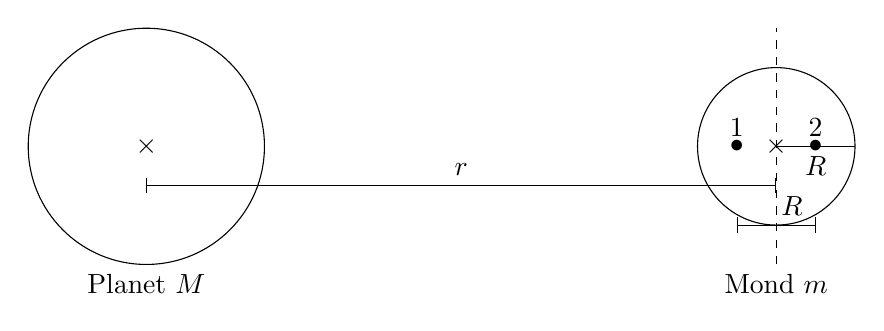
\begin{tikzpicture}
        \draw (0,0) circle (1.5) node {$\times$};
        \node [below] at (0,-1.5) {Planet $M$};
        \draw (8,0) circle (1.0) node {$\times$};
        \node [below] at (8,-1.5) {Mond $m$};
        \draw [dashed] (8, -1.5) -- (8, 1.5);
        \draw [|-|] (0,-0.5) -- (8,-0.5) node [pos=0.5, above] {$r$};
        \draw [|-|] (7.5,-1) -- (8.5,-1) node [pos=0.7, above] {$R$};
        \draw (8, 0) -- (9, 0) node [pos=0.5, below] {$R$};
        \node [above] at (7.5,0) {$1$};
        \node at (7.5,0) {$\bullet$};
        \node [above] at (8.5,0) {$2$};
        \node at (8.5,0) {$\bullet$};
    \end{tikzpicture}
\end{center}
\begin{align*}
    r_1 &= r - \frac{R}{2} \\
    r_2 &= r + \frac{R}{2}
\end{align*}

\paragraph{Betrachte}
\begin{enumerate}[i)]
    \item Gravitationskraft: "`Hälften"'
        \[ F_M = - G \frac{m}{2} \frac{m}{2} \frac{1}{R^2} \]
        $\rightarrow$ bestimmt den "`Zusammenhalt des Mondes"'
        (Vernachlässigung der Festkörpereigenschaften!!!)
    \item Unterschiedliche Gravitationskräfte eines 2. Körpers (Planet) auf
        die beiden "`Hälften"'
        \begin{align*}
            F_1 &= -G M \frac{m}{2} \frac{1}{r_1^2} = \frac{GMm}{2} \frac{1}{\left(r-\frac{R}{2}\right)^2}
            F_2 &= -G M \frac{m}{2} \frac{1}{r_2^2} = \frac{GMm}{2} \frac{1}{\left(r+\frac{R}{2}\right)^2}
        \end{align*}
\end{enumerate}

\begin{definition}
    Gezeitenkraft
    \[ F_{\mathrm{Gez}} = F_1 - F_2 = - \frac{GMm}{2} \left(\frac{1}{\left(r-\frac{R}{2}\right)^2} - \frac{1}{\left(r+\frac{R}{2}\right)^2}\right) \]
\end{definition}

\paragraph{Allgemein} $r \gg R$ (gilt \emph{nicht} für enge Doppelsterne)

Reihenentwicklung:
\[ \frac{1}{x^2} = \frac{1}{x_0^2} - \frac{2}{x_0^3} (x-x_0) + 0\]
\begin{align*}
    \frac{1}{\left(r - \frac{R}{2}\right)^2} &= \frac{1}{r^2} + \frac{1}{r^3} R\\
    \frac{1}{\left(r + \frac{R}{2}\right)^2} &= \frac{1}{r^2} - \frac{1}{r^3} R\\
    \Rightarrow F_{\mathrm{Gez}} &= -\frac{GMm}{2} \left(\frac{R}{r^3} + \frac{R}{r^3}\right) = G M m \frac{R}{r^3}
\end{align*}

\paragraph{Bedingung} Stabilität: $|F_m| > |F_{\mathrm{Gez}}|$
\[ \frac{4M}{m} < \left(\frac{r}{R}\right)^3 \Leftrightarrow \frac{m}{4M} > \left(\frac{R}{r}\right)^3 \]
\begin{align*}
    M &= \bar \rho_{\mathrm{Pl}} \cdot \frac{4}{3} \pi R_{\mathrm{m}}^3 & m &= \bar \rho_{\mathrm{Pl}} \cdot \frac{4}{3} \pi R^3
\end{align*}
\[ \Rightarrow r > \sqrt[3]{4 \frac{\bar \rho_{\mathrm{Pl}}}{\bar \rho_{m}}} \cdot R_{\mathrm{Pl}} \]
Genaure Rechnung liefert: \textsc{Roche}-Grenze
\[ \Rightarrow r > \sqrt[3]{\frac{\bar \rho_{\mathrm{Pl}}}{\bar \rho_{m}}} \cdot 2.44 \cdot R_{\mathrm{Pl}} \]

\section{Bedingungen für Planetenentstehung}
Entstehung aus Staub-/Gasscheiben von jungen Sternen $\rightarrow$ Beispiel: $\beta$ Pic

\paragraph{Szenario} Sonnensystem
\begin{itemize}
    \item Sternwind $T$ im inneren Sonnensystem hoch
    \item Sternwind $T$ im äußeren Sonnensystem niedrig \\
        $\Rightarrow$ Akkredition von Restgas
    \item Ausdünnung der Scheibe nach außen
    \item kleine Gesteinsplaneten innen
    \item große Planeten mittig
    \item Gasplaneten weiter außen
    \item Kometen ganz außen
\end{itemize}

\paragraph{Prolem} Neue Planetenklasse

``Hot Jupiter'': sehr massereiche Gasplaneten nah am Stern

$\Rightarrow$ konkurierende Entstehungstheorien:
\begin{itemize}
    \item \framebox{in situ}
    \item \framebox{Migration}
\end{itemize}
